\begin{frame}
\frametitle{Présentation du dispositif expérimental}
Afin de mesurer les chocs subits par le coureur on réalise une semelle particulière dotée de:
\begin{itemize}
\item 4 capteurs de pression
\item Un lecteur de carte SD
\item Un microcontrolleur
\end{itemize}
\end{frame}

\begin{frame}
\frametitle{Le capteur de pression (ref ici)}
Le capteur de pression est une résistance de variable de loi non linéaire.

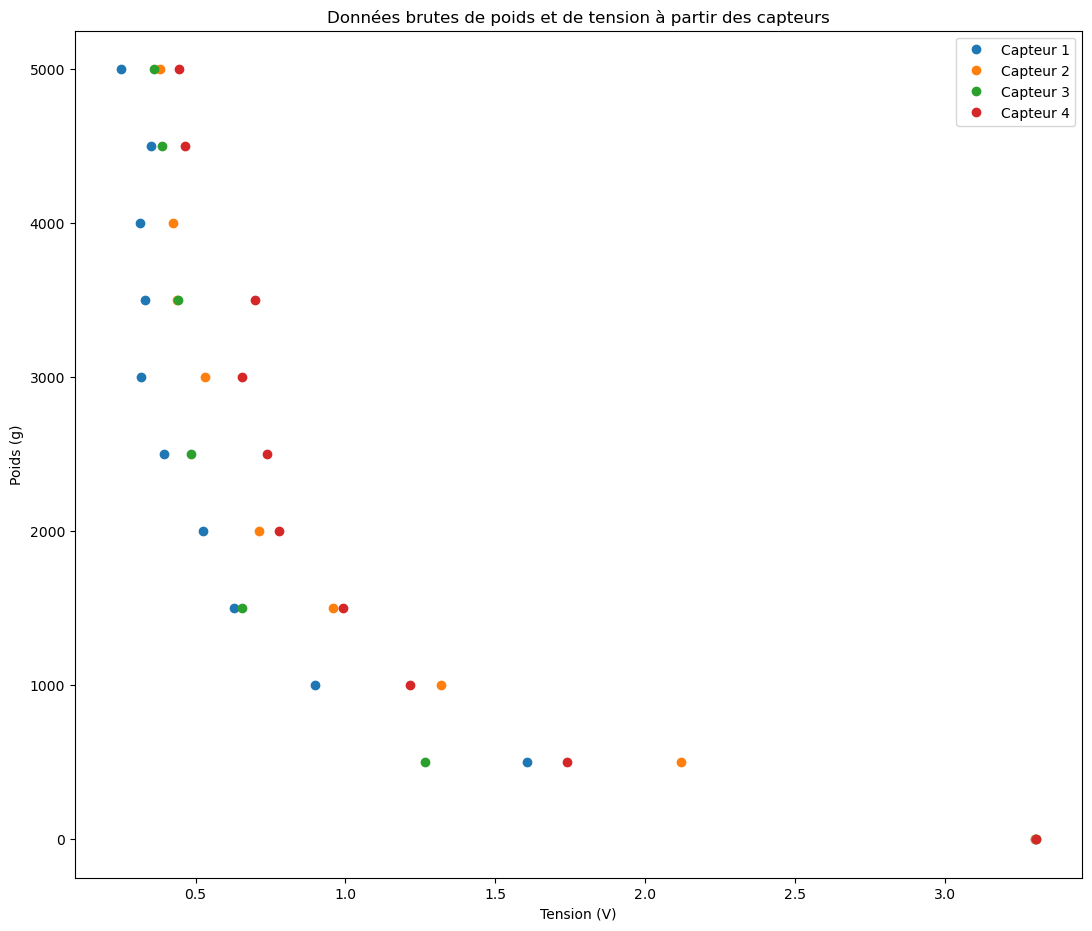
\includegraphics[scale=0.3]{./figures/cal_00.png}
\end{frame}

\begin{frame}
\frametitle{Carte de contrôle}
Voici la carte avec le microcontroleur, les convertisseurs analogiques-numériques et le lecteur de carte SD:
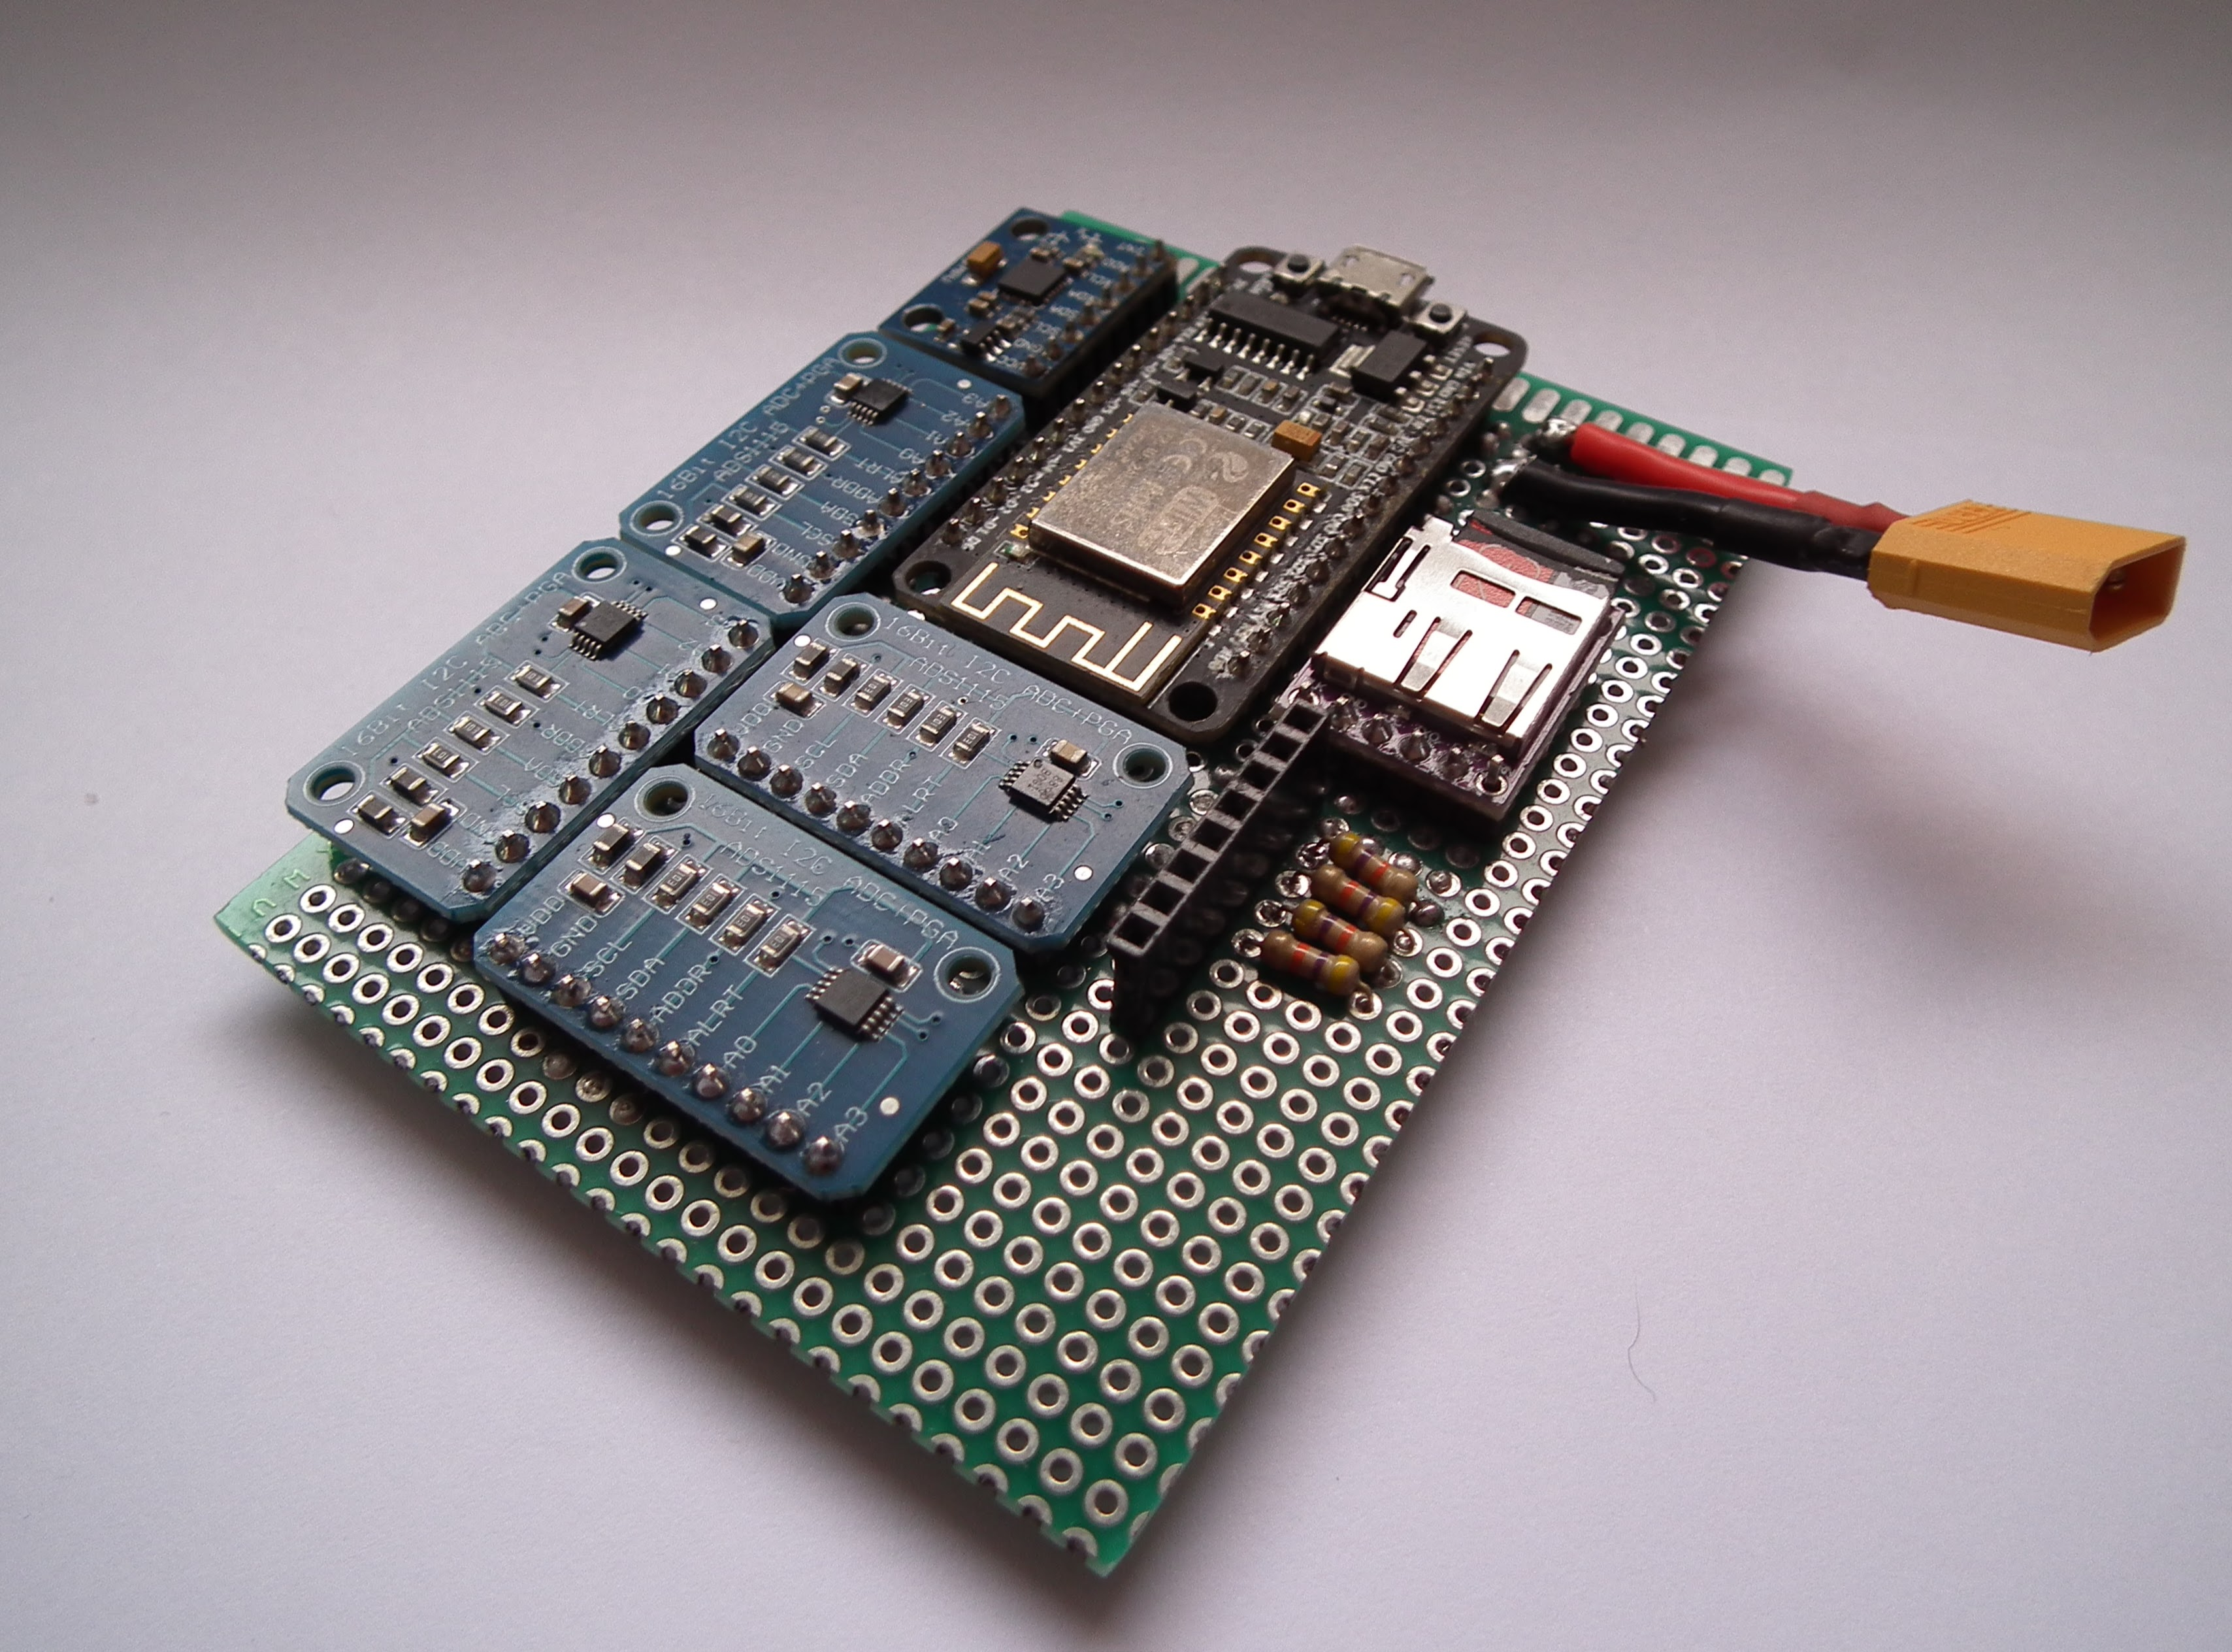
\includegraphics[width=\textwidth]{./figures/carte_00.jpg}

\end{frame}

\begin{frame}
\frametitle{Calibration - ajustement de courbe}

\end{frame}

\begin{frame}
\frametitle{Calibration - résultats 1/2}
Résultat de la méthode des moindres carrés avec la descente de gradient effectué sur la carte:\\
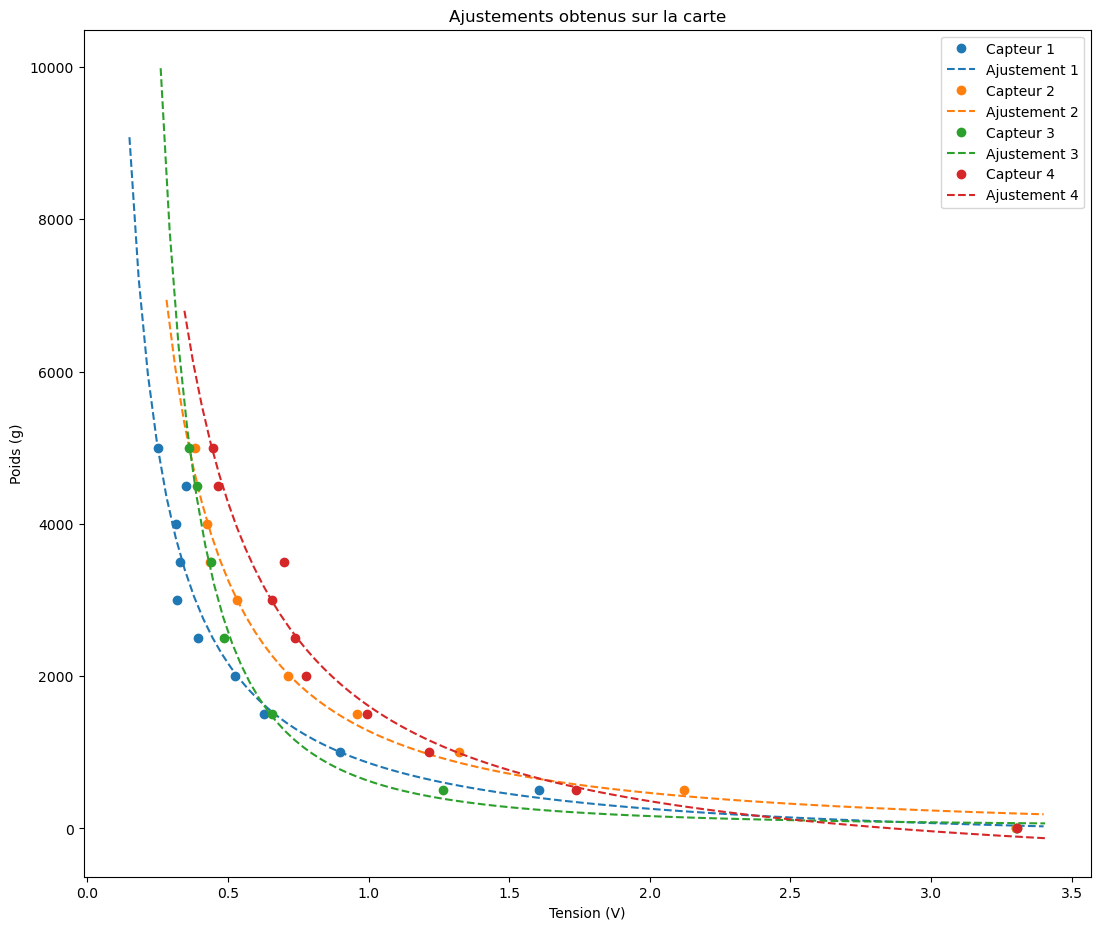
\includegraphics[scale=0.3]{./figures/cal_01.png}
\end{frame}

\begin{frame}
\frametitle{Calibration - résultats 2/2}
Comparaison avec la fonction \texttt{curve\_fit} de \texttt{scipy}:\\
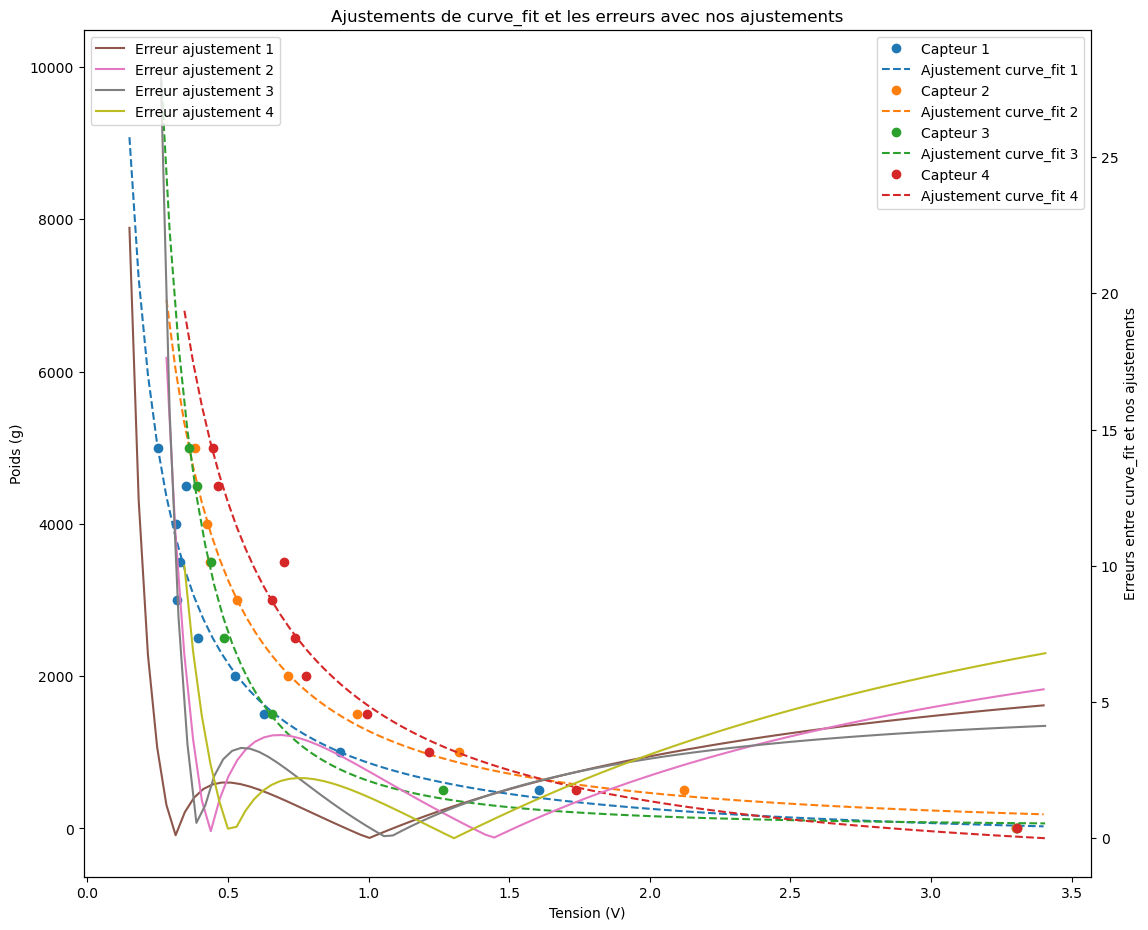
\includegraphics[scale=0.3]{./figures/cal_02.png}
\end{frame}


\begin{frame}
\frametitle{La semelle}
Voici les capteurs disposés sur la semelle
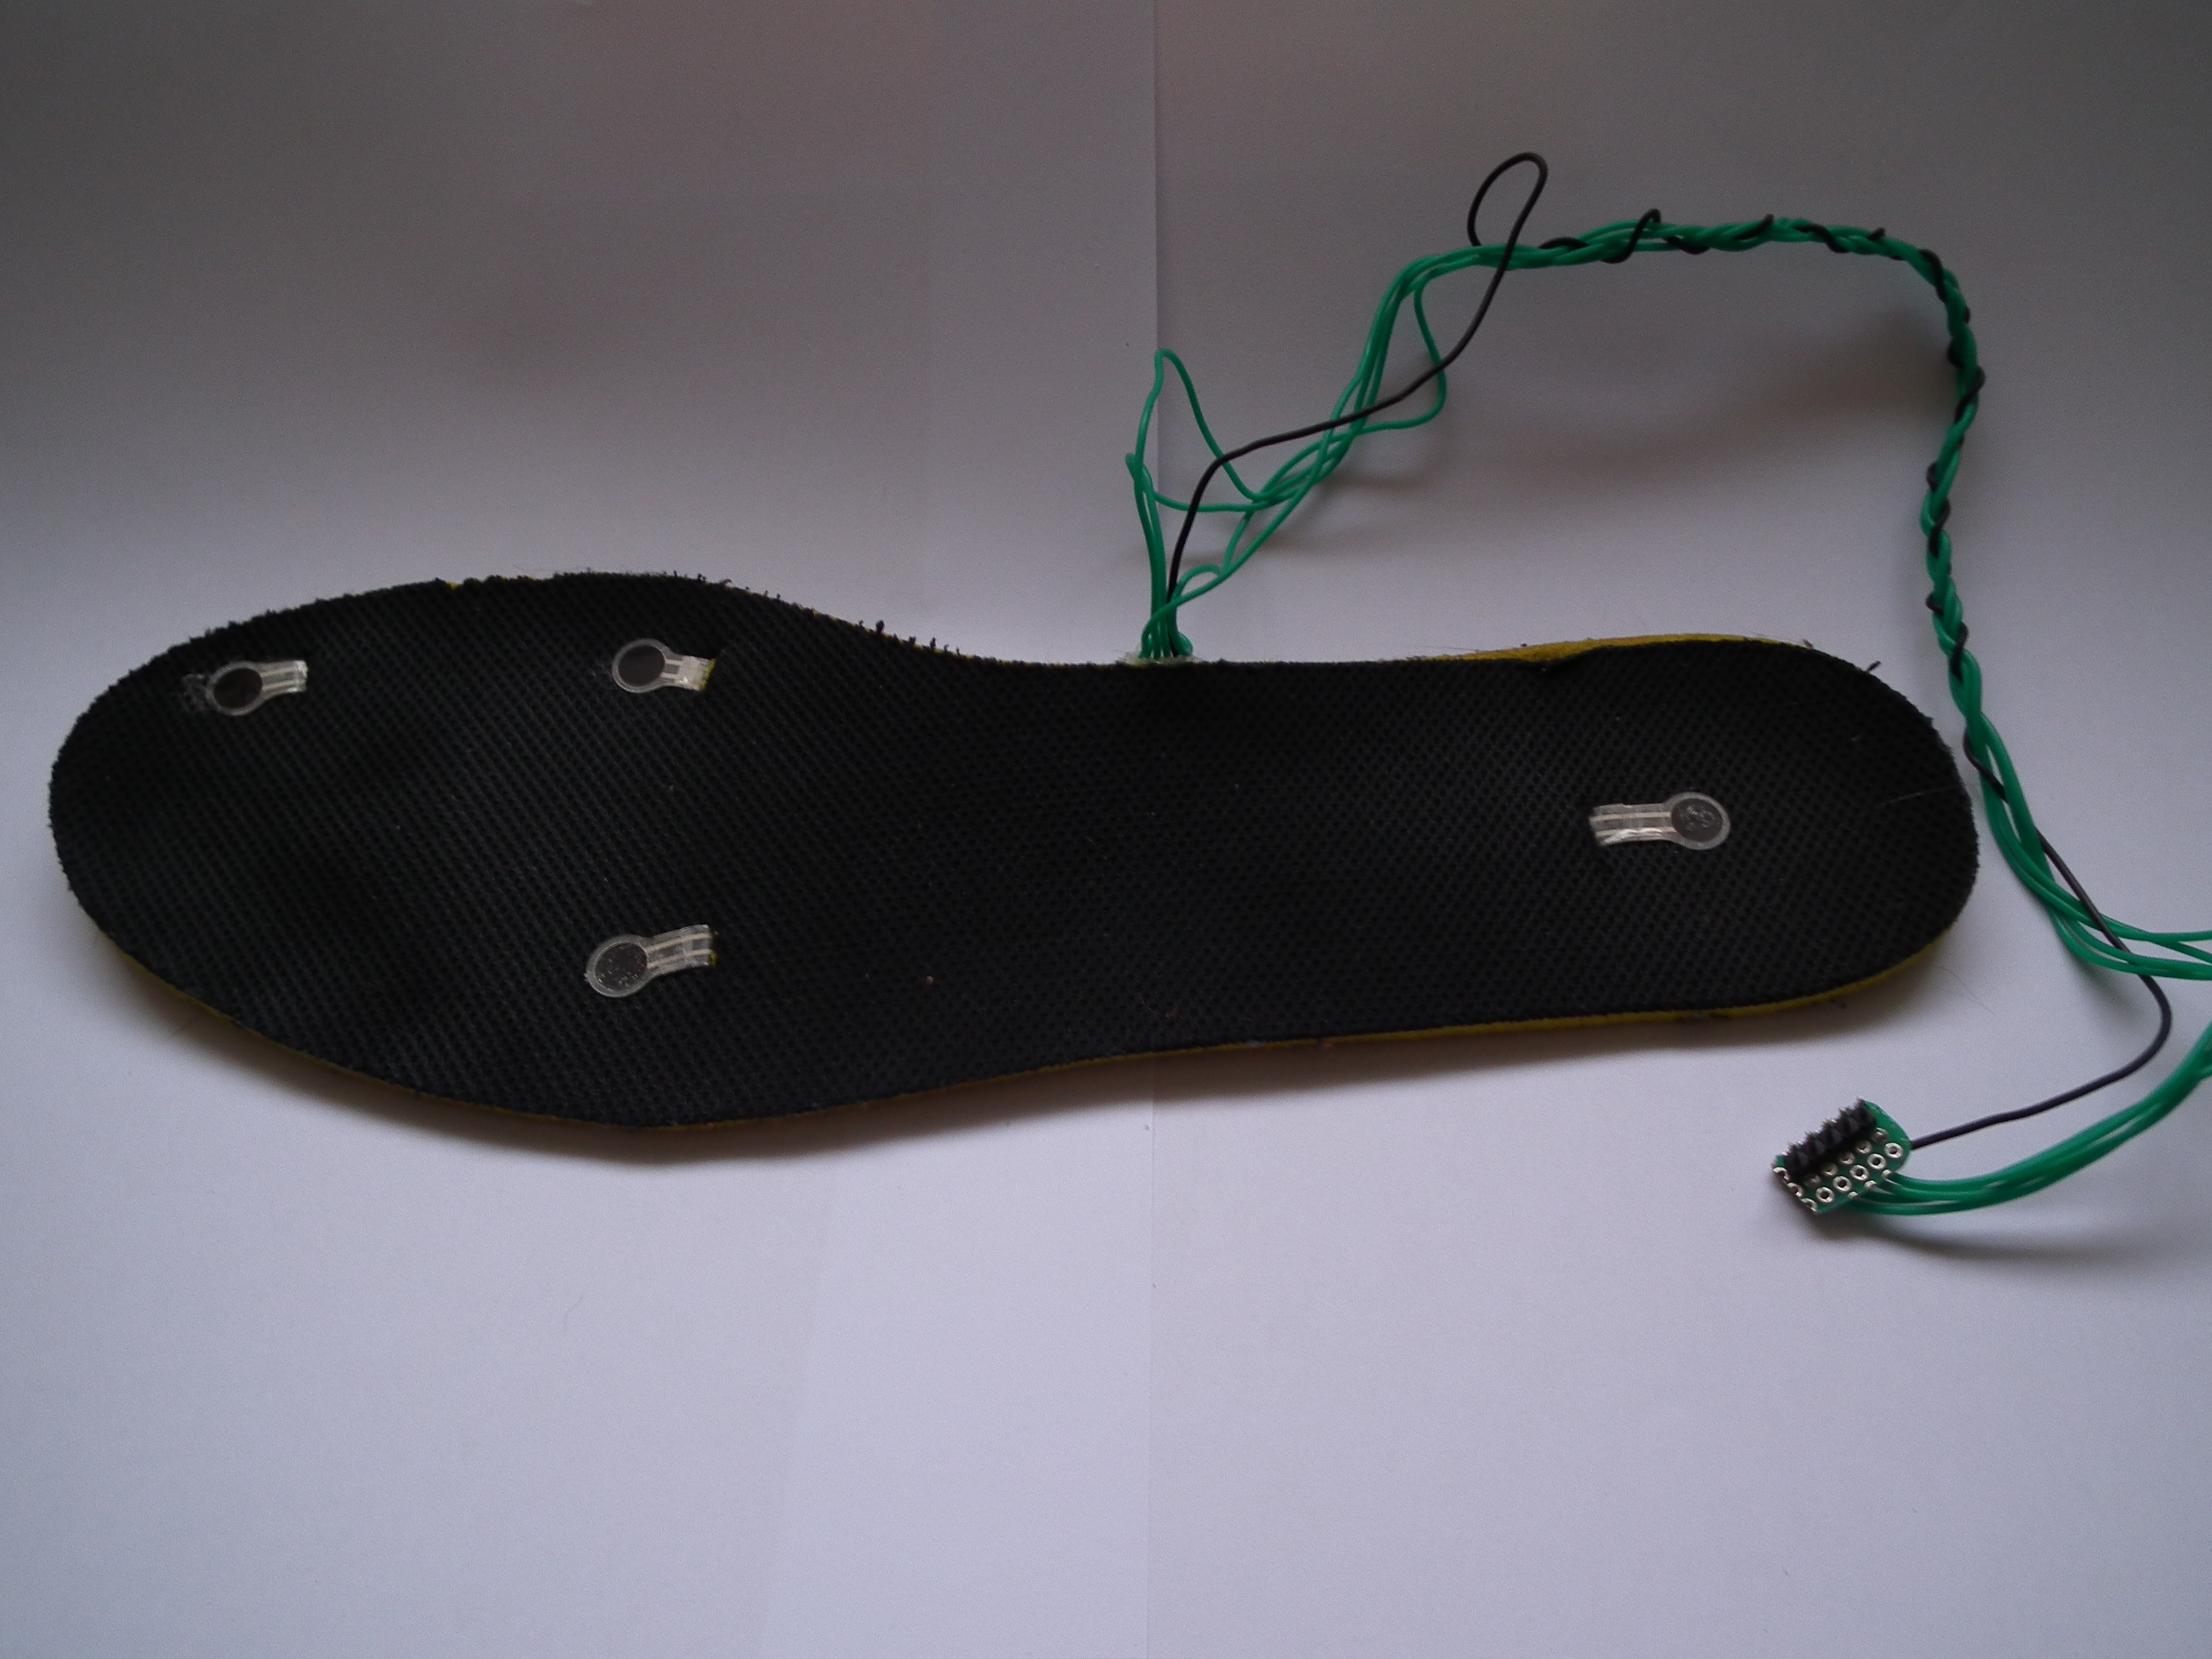
\includegraphics[width=\textwidth]{./figures/sem_00.jpg}

\end{frame}

\begin{frame}
\frametitle{Les premiers résultats}

\end{frame}
